\subsection{Schwarz-Christoffel}
Thus the Riemann Mapping Theorem gives us a biholomorphism between the unit disk and the interior of a polygon (which in fact extends to a homeomorphism on the closures of these spaces). Now that we know such a function exists, we would like to know what it is. As it turns out, we can give an explicit formula for it or more precisely for its inverse.
\begin{theorem}[Schwarz-Christoffel Formula]
    The functions $z = F(w)$ which map $\abs{w} < 1$ conformally to a polygon $\Omega$ with angles $\alpha_k \pi$ for $k = 1, \dots, n$ are of the form 
    $$F(w) = c \int_0^w \prod_{k = 1}^n (w - w_k)^{-\beta_k} dw + c' $$
    where $c, c'$ are some complex constants (as one can guess they determine the scaling and translation) and the $w_k$ are the images of the vertices $z_k$ (hence $w_k$ lie on the unit circle).
\end{theorem}
\begin{remark}
    The integral is evaluated by integrating along any path from 0 to $w$. Because the disk is simply connected this is well-defined.
\end{remark}
\begin{proof}
    Let $\Omega$ be the interior of a polygon. In order to verify the formula, we want to show that if $F$ is the inverse of a biholomorphism $f: \Omega \to D$ given by the Riemann mapping theorem then
    $$F'(w) = c \prod_{k = 1}^n (w - w_k)^{-\beta_k}$$

    Consider $w = g(\zeta) = f(z_k + \zeta^{\alpha_k})$ as we did before. Notice that this is invertible near $\zeta = 0$ (the local extensions below the half-plane are injective). In particular there is a Taylor series expansion 
    $$\zeta = \sum_{n = 0}^\infty b_n (w - w_k)^n$$
    By construction, $b_0 = 0$ and $b_1 \neq 0$. Therefore 
    \begin{align*}
        \zeta = \sum_{n = 1}^\infty b_1 (w - w_k)^n = (w - w_k) \underbrace{\left( \sum_{n = 0}^\infty b_{n + 1} (w - w_k)^n \right)}_{g_k(w)}
    \end{align*}
    where $g_k(w)$ is non-zero around $w = w_k$. Since $z = z_k + \zeta^{\alpha_k}$ we have 
    $$z = F(w) = z_k + (w - w_k)^{\alpha_k} g_k(w)^{\alpha_k}$$
    Relabeling $g_k(w)^{\alpha_k} = g_k(w)$, we have 
    \begin{align*}
        F'(w) = \alpha_k (w - w_k)^{\alpha_k - 1} g_k(w) + (w - w_k)^{\alpha_k} g_k'(w)
    \end{align*}
    Since $\beta_k = 1 - \alpha_k$ we can write 
    \begin{align*}
        F'(w) (w - w_k)^{\beta_k} = \alpha_k g_k(w) + (w - w_k)g_k'(w)
    \end{align*} 
    implying that $F'(w)(w - w_k)^{\beta_k}$ is non-vanishing around $w_k$. Notice that $F'(w)$ is non-zero away from the vertices since $f$ is conformal at these points. Therefore 
    $$H(w) = F'(w) \prod_{k = 1}^n (w - w_k)^{\beta_k}$$
    is holomorphic and vanising in a neighbourhood of $\ol{D}$. 

    We claim that $H(w)$ is actually constant. We first show that $\arg H(w)$ is constant on $S^1$. We observe first that
    $$ \frac{d}{d\theta} F(e^{i\theta}) = F'(e^{i\theta}) i e^{i\theta} $$
    Taking arguments of both sides we have 
    $$ \arg \left( \frac{d}{d\theta} F(e^{i\theta}) \right) = \arg (F'(e^{i\theta})) + \left( \theta + \frac{\pi}{2} \right)$$
    We claim the left hand side is constant. In order to see this, consider $e^{i \theta}$ between $w_k$ and $w_{k + 1}$. Notice that $F(e^{i \theta})$ describes a straight line so we can write 
    $$F(e^{i \theta}) = \alpha t(\theta) + \beta$$
    where $t$ is a real-valued function of $\theta$ and $\alpha, \beta$ are constants. Then 
    $$ \arg \left( \frac{d}{d\theta} F(e^{i \theta}) \right) = \arg (\alpha t'(\theta)) = \arg (\alpha ) $$
    
    \begin{figure}[ht]
        \centering
        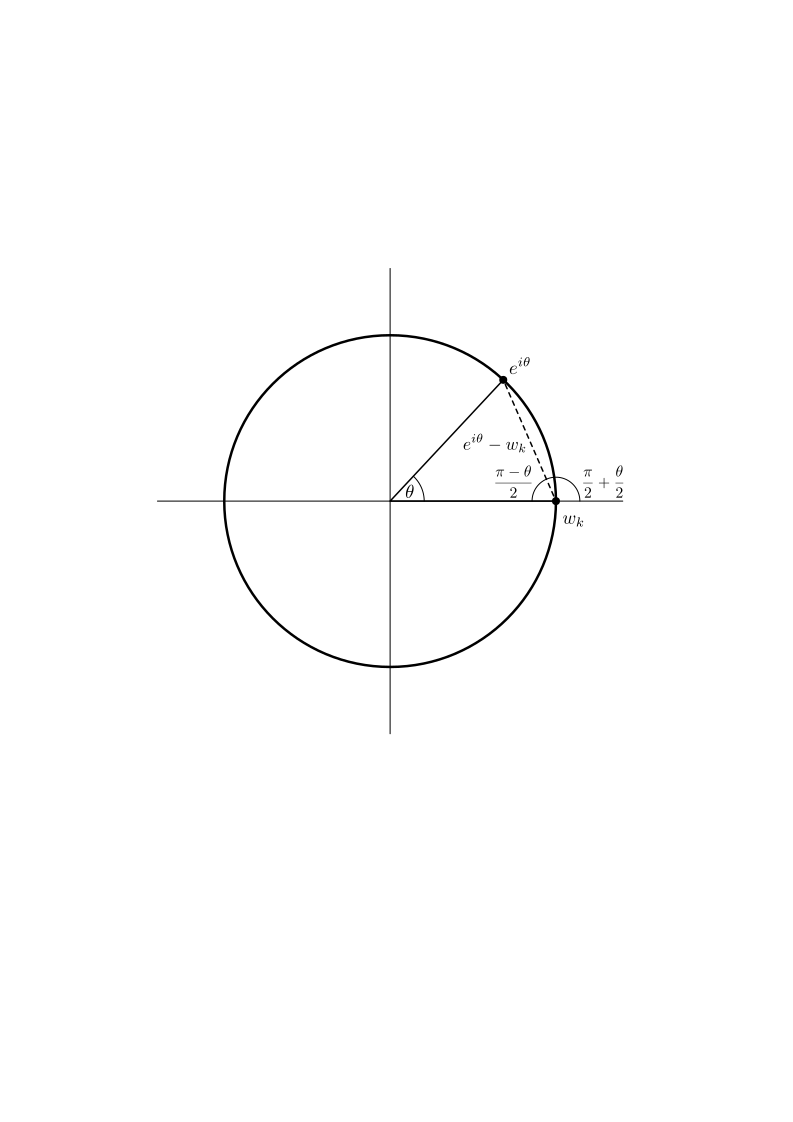
\includegraphics[scale=0.9]{Images/schwarz_christoff_arg.png}
        \caption{The argument of $e^{i \theta} - w_k$ is $\theta/2 + \text{const}$}
        \label{fig:schwarz-christoff-arg}
    \end{figure}

    Additionally by \autoref{fig:schwarz-christoff-arg} we see that $\arg(e^{i \theta} - w_k) = \theta/2 + \text{const}$. Then 
    \begin{align*}
        \arg H(e^{i \theta}) = - \theta + \left(\sum_{k = 1}^n \beta_k \right) \frac{\theta}{2} + \text{const}
    \end{align*}
    Since $\sum \beta_k = 2$ by assumption, we see that $\arg H(e^{i \theta})$ is constant. By the mean value property, we conclude that $H(0)$ is exactly this constant. But then the maximum modulus principle implies that $H$ must be constant on the entire closed disk. This means that 
    $$F'(w) = c \prod_{k = 1}^n (w - w_k)^{-\beta_k}$$
    Integrating both sides, we get the formula.
\end{proof}

\subsection{Examples}
Above we worked out the Schwarz-Christoffel formula for the disk. But since we have an explicit biholomorphism between the disk and the upper half-plane, we can translate the formula to the upper half-plane by performing a substitution $w = (\zeta - i)/(\zeta + i)$. In fact the formula remains the same after this substitution (things cancel out in a lovely way) with the $w_k$ being real numbers. 

We can then use this formula to give an explicit mapping from the upper half plane to a rectangle. First we need to choose 4 points on the real axis that will map to the four vertices of the rectangle. We will take these four points to be $1, -1, 1/k, -1/k$ for some $0 < k < 1$. Then according to the formula 
$$ z = F(w) = \int_0^w \frac{dw}{\sqrt{(1 - w^2)}\sqrt{1 - k^2 w^2}} $$
maps the upper half-plane to the rectangle with vertices $K, K + iK', -K + iK', -K$ where 
$$K = \int_0^1 \frac{dt}{(1 - t^2)(1 - k^2t^2)}$$
and 
$$K' = \int_1^\infty \frac{dt}{(1 - t^2)(1 - k^2t^2)}$$
(see \autoref{fig:H-to-rect} for reference).
The inverse map $w = f(z)$ is a conformal map from the rectangle to the upper-half plane. We can extend this map beyond the rectangle to the entire plane by repeatedly reflecting across its sides. This defines a double periodic, meromorphic function on $\C$ with group of periods generated by $4K, 2iK'$

\begin{figure}[ht]
    \centering
    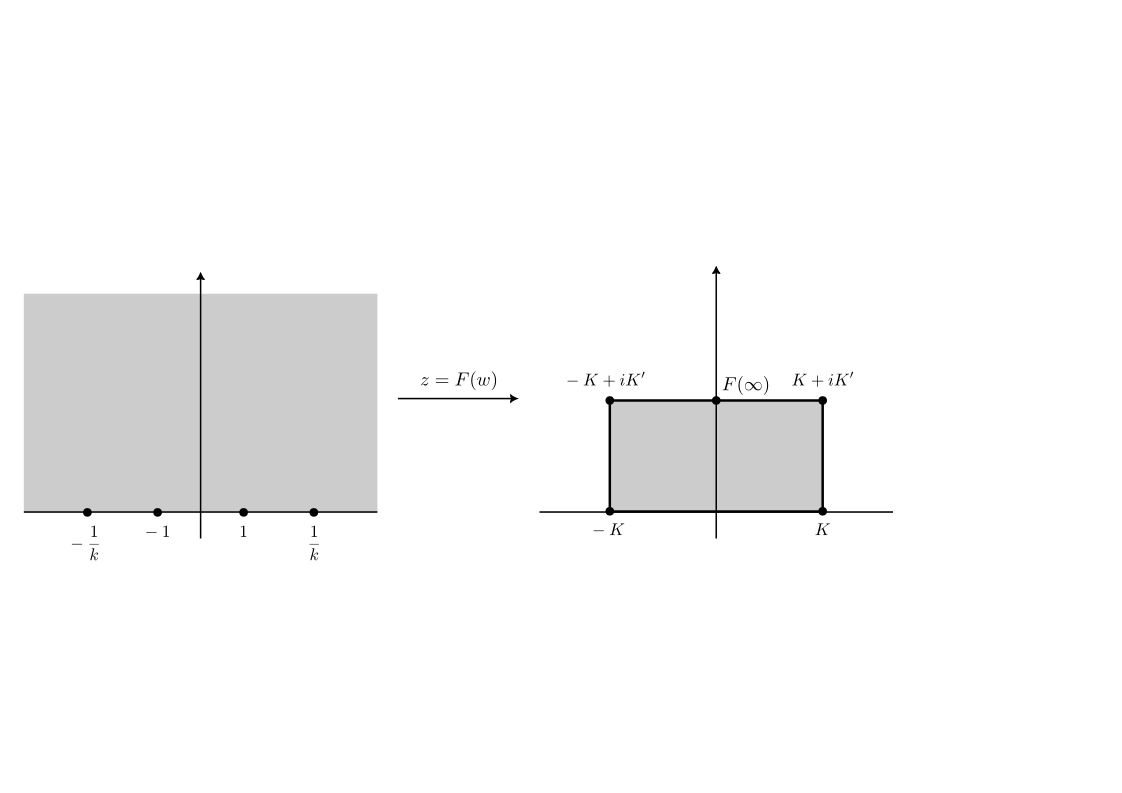
\includegraphics[scale=0.7]{Images/H_to_rect.png}
    \caption{Mapping upper half-plane to a rectangle}
    \label{fig:H-to-rect}
\end{figure}
% TODO: Add diagram

\secbreak

We can do the same thing with a triangle with angles $\alpha_1 \pi, \alpha_2 \pi, \alpha_3 \pi$. We will choose our three points on the real axis to be $0, 1$ and $\infty$. Then the map is 
$$z = F(w) = \int_0^w w^{\alpha_1 - 1}(w - 1)^{\alpha_2 - 1}$$

The inverse defines a map from the triangle to the upper half plane and we can ask again whether this map can be extended to the entire plane by reflection. In order for the reflections to line up, we would need to be able to able to tile the entire plane with these triangles in such a way that there are an even number of triangles around every vertex. Therefore we have $\alpha_k \pi = 2\pi/2n_k$ for integers $n_k$. Then since the sum of the $\alpha_k$ is 1 in a triangle we have 
\begin{align*}
    \frac{1}{n_1} + \frac{1}{n_2} + \frac{1}{n_3} = 1
\end{align*}
One can then verify that there are only 3 sets of natural numbers satisfying this. Namely, $(3, 3, 3), (2, 4, 4)$ and $(2, 3, 6)$. 

\section{Normal families of Meromorphic Functions}
Much like we did with holomorphic functions, we want to find the normal families (i.e. the (pre)compact subsets) of the collection of meromorphic functions. One can simply think of meromorphic functions as functions that take values in $S^2$ instead of just $\C$. A nice way to `deal with' $S^2$ is the previously mentioned chordal metric. Recall that the chordal metric is the Euclidean distance in $\R^3$ between two points on the Riemann sphere under the usual stereographic projection map and is given by 
$$d(z, w) = \frac{2\abs{z - w}}{\sqrt{1 + \abs{z}^2} \sqrt{1 + \abs{w}^2}}$$
for $z, w \neq \infty$. As mentioned previously, an important property of the chordal metric is that $d(z, w) = d(1/z, 1/w)$ (which also tells us how the find the distance between finite points and the point at infinity). 

Of course our starting point when studying normal families is the \hyperref[thm:arzela-ascoli]{Arzelà–Ascoli theorem}, which tells us that a family of continuous functions with values in the Riemann sphere \textit{equipped with the chordal metric} is normal if and and only if it is equicontinuous (every function is automatically bounded since the chordal metric is itself at most 2).

\begin{lemma}\label{lem:conv-merom-or-inf}
    Let $\{f_n\}$ be a sequence of meromorphic function on a domain $\Omega$ which converges uniformly on compact sets with respect to the chordal metric. Then the limit $f$ is either meromorphic or identically $\infty$.
\end{lemma}
\begin{proof}
    Let $z_0 \in \Omega$ be arbitrary. Suppose $\abs{f(z_0)} < \infty$. Then $f$ is bounded in a neighbourhood of $z_0$. This means that $f_n \to f$ on compact sets in a neighbourhood of $z_0$ with respect to the Euclidean metric (because the two metrics are equivalent on bounded subsets of $\C$). This means that $f$ is holomorphic on a neighbourhood of $z_0$.

    Alternatively we might have $f(z_0) = \infty$, then we simply repeat the above argument with $\{1/f_n\}$ instead. In particular, $\{1/f_n\}$ are bounded in a neighbourhood of $z_0$ for $n$ large enough. So $1/f$ is holomorphic in a neighbourhood of $z_0$ and $1/f$ is 0 at $z_0$. Either the zeroes of $1/f$ are isolated (in which case $f$ is meromorphic) or $1/f$ is identically 0 in a neighbourhood of $z_0$. 
\end{proof}

\begin{example}
    The sequence $\{z_n\}$ converges uniformly on compact subsets in the complement of $\ol{D}$ to $\infty$. 
\end{example}

\begin{corollary}\label{cor:conv-holom-or-inf}
    Let $\{f_n\}$ be a sequence of holomorphic functions on a domain $\Omega$ which converges uniformly on compact sets with respect to the chordal metric. Then the limit $f$ is either holomorphic or identically $\infty$.
\end{corollary}
\begin{proof}
    Done in an assignment.
\end{proof}

What we would like to do is generalise \hyperref[thm:montel-thm]{Montel's Theorem} to work for meromorphic functions. For this we will need to introduce the spherical derivative.
\subsection{Spherical Derivative}
\begin{definition}[Spherical Derivative]
If $f$ is a meromorphic function defined on a domain $\Omega \subset \C$, then the \textit{spherical derivative} of $f$ is defined by
\begin{align*}
    f^\#(z) := \lim_{w \to z} \frac{d(f(z), f(w))}{\abs{z - w}}
\end{align*}
where of course by $d$ we mean the chordal metric. 
\end{definition}

Therefore the spherical derivative is always a non-negative real number. If we take $\Omega$ to be a subset of the Riemann sphere, then we use the chordal metric in the denominator as well. Notice that if $z$ is not a pole then using the definition of the chordal metric we have
\begin{align*}
    f^\#(z) &= \lim_{w \to z} \frac{d(f(z), f(w))}{\abs{z - w}}\\
    &= \lim_{w \to z} \frac{1}{\abs{z - w}} \cdot \frac{2\abs{f(z) - f(w)}}{\sqrt{1 + \abs{z}^2} \sqrt{1 + \abs{w}^2}}\\
    &= \lim_{w \to z} \frac{\abs{f(z) - f(w)}}{\abs{z - w}} \cdot \frac{2}{\sqrt{1 + \abs{z}^2} \sqrt{1 + \abs{w}^2}}\\
    &= \frac{2\abs{f'(z)}}{1 + \abs{f(z)}^2}
\end{align*}

This is a very useful formula as it relates the spherical derivative with the true derivative. For example, we can use it to find a version of the chain rule for spherical differentiation.
\begin{align*}
    (f \circ g)^\#(z) = \frac{2 \abs{(f \circ g)'(z)}}{1 + \abs{(f \circ g)(z)}^2} = \frac{2 \abs{f'(g(z))}}{1 + \abs{f(g(z))}^2} \abs{g'(z)} = f^\#(g(z)) \abs{g'(z)}
\end{align*}

Despite always being a real number (and always a non-negative one at that), the spherical derivative can still give us a fair bit of information. For example by the calculation above we see that if $f^\#(z) \neq 0$ then $f'(z) \neq 0$ so we know that $f$ is locally 1-1. Moreover, by properties of the chordal metric, we have that $f^\# = (1/f)^\#$. This identity allows us to find the spherical derivative at poles. In fact this means that $f^\#$ is a continuous function on all of $\Omega$, including the poles. The spherical derivative is what allows us to generalise Montel's Theorem to a statement about meromorphic functions.

\begin{theorem}[Marty's Theorem]\label{thm:marty}
    A family of meromorphic functions $\scrS$ on a domain $\Omega$ is normal (with respect to the chordal metric) if and only if $\scrS^\# := \{f^\# : f \in \scrS\}$ is locally bounded.
\end{theorem}
\begin{proof}
    First suppose $\scrS$ is a normal family of meromorphic functions and suppose $\scrS^\#$ is not locally bounded. Because the Euclidean metric and chordal metric are equivalent on bounded subsets of $\C$, they share the same normal families (assuming no poles). We will use this along with the relationship between $f^\#$ and $f'$ to get a contradiction.
    
    Since $\scrS^\#$ is not locally bounded, there exists a point $z_0 \in \Omega$ such that $\scrS^\#$ is not bounded in any neighbourhood of $z_0$. This means there exists a sequence of functions $f_n \subset \scrS$ and a sequence of points $z_n \to z_0$ such that $f_n^\#(z_n) \to \infty$. By normality we can assume that this sequence of functions converges to some meromorphic function $f$ (passing to a subsequence if necessary). Then we know by \autoref{lem:conv-merom-or-inf} that $f$ is either meromorphic or identically infinity. 
    
    Suppose $f$ is bounded at $z_0$. It is then bounded in a neighbourhood $U$ of $z_0$. We can take $U$ to be a bounded subset of $\C$ so that the $f_n$ in fact converge to $f$ on $U$ in the Euclidean metric. Then $f_n'(z_0) \to f'(z_0)$. But then $f_n^\#(z_0) \to f^\#(z_0)$ leading to a contradiction. If $f$ is not bounded at $z_0$, we can repeat the argument with $1/f$. 

    In order to see the converse, suppose $\scrS^\#$ is locally bounded. Let $z_0 \in \Omega$ be arbitrary and let $D$ be a closed disk centered at $z_0$ so that $\{f^\# : f \in \scrS\}$ is bounded by $M$ on $D$. By definition this means that 
    \begin{align*}
        \lim_{z \to w} \frac{d(f(z), f(w))}{\abs{z - w}} \leq M
    \end{align*}
    In particular for $w$, there exists a $\delta_w$ such that if $\abs{z - w} < \delta_w$ then $d(f(z), f(w))/\abs{z - w} < 2M$ or in other words $d(f(z), f(w)) < 2M \abs{z - w}$. We cover $D$ by such neighbourhoods (notice that the size of the neighbourhoods may vary with $w$). Let $\delta$ be a Lebesgue number for this covering (which exists by compactness of $D$) so that $\{\abs{z - w} < \delta\} \subset \{\abs{z - w} < \delta_w\}$ for all $w \in D$. 

    Now let $w, w'$ be arbitrary points in $D$. Connect them via a line segment and partition the line $\{w_0, \dots, w_{n}\}$ with $w_0 = w$ and $w_{n} = w'$ such that $\abs{w_{j + 1} - w_j} < \delta$ (see \autoref{fig:marty-thm}). Then 
    \begin{align*}
        d(f(w'), f(w)) &\leq \sum_{j = 1}^n d(f(w_{j}), f(w_{j - 1}))\\
        &< 2M \sum_{j = 1}^n \abs{w_j - w_{j - 1}}\\
        &= 2M \abs{w' - w}
    \end{align*}
    Therefore all the $f$ in $\scrS$ are in particular Lipschitz with Lipschitz constant $2M$ and hence $\scrS$ is equicontinuous on $D$ (with respect to the chordal metric) and hence form a normal family by the \hyperref[thm:arzela-ascoli]{Arzelà–Ascoli Theorem}. Since the collection of such disks cover $D$, we conclude that by the `suitable cover lemma' (see \autoref{lem:suitable-cover}) that $\scrS$ is itself a normal family on $\Omega$. 

    \begin{figure}[ht]
        \centering
        \includegraphics[scale=0.7]{Images/marty_thm.png}
        \caption{Partition the line segment connecting $w$ and $w'$}
        \label{fig:marty-thm}
    \end{figure}
\end{proof}

\begin{theorem}[Picard's Big Theorem]
    If $f(z)$ is holomorphic with an essential singularity at $z_0$, then there exists $\lambda \in \C$ such that in any neighbourhood $z_0$, $f$ assumes every value except maybe $\lambda$ (infinitely many times).

    Equivalently, if $f(z)$ is meromorphic in a punctured disk $0 < \abs{z - z_0} < \delta$ and $f$ omits 3 values in $\C \cup \{\infty\}$, then $f$ is meromorphic in $\abs{z - z_0} < \delta$.
\end{theorem}
\begin{proof}[Proof of equivalence]
    We first show why the above statements are equivalent. Suppose the first statement about holomorphic functions holds. Then by composing with an FLT if necessary we can assume that $f$ omits $\infty$ and 2 other (finite) values. Then $f$ on $0 < \abs{z - z_0} < \delta$ is a holomorphic function that misses 2 values which means that $z_0$ cannot be an essential singularity of $f$ and therefore must be a pole.

    Now suppose the statement about meromorphic functions holds. Let $f$ be an entire function and $z_0$ an essential singularity. Consider $f$ on $0 < \abs{z - z_0} < \delta$ (for any $\delta$. Notice that such a punctured disk is contained in every punctured neighbourhood of $z_0$). Then $f$ omits the value $\infty$ on this punctured disk (since it is holomorphic). Then if it missed 2 more distinct complex numbers we could conclude that $f$ is meromorphic on the entire disk which we know is not true. Therefore $f$ can miss at most one more value.
\end{proof}

We will see that Picard's Big Theorem is in fact a fairly straightforward consequence of Montel's Big Theorem.
\begin{theorem}[Montel's Big Theorem]
    A family of meromorphic functions on a domain $\Omega$ which omits 3 distinct values in $\C \cup \{\infty\}$ is normal in the chordal metric.
\end{theorem}
